\chapter{AES}

Phần này tham khảo chính từ \cite{Stallings}.

AES biến đổi theo khối 128 bit, sử dụng mô hình mạng SPN.

Bốn phép biến đổi chính là Add Round Key, Substitute Bytes, Shift Rows và Mix Columns.

Quá trình giải mã sử dụng phép biến đổi ngược của 4 phép biến đổi trên là Inverse Sub Bytes, Inverse Shift Rows, Inverse Mix Columns. Đối với Add Row Key bản thân là phép xor nên phép biến đổi ngược là chính nó.

AES hỗ trợ key với các kích thước: 128 bit, 192 bit và 256 bit. AES dùng hàm Expand Key để mở rộng khóa thành 44 word 32 bit với key 128 bit thành 11 cụm khóa con. Mỗi 4 word làm tham số cho một phép Add Row Key.

Mỗi block bản rõ 16 byte $p_0, p_1, \ldots, p_{15}$ được tổ chức dưới dạng một ma trận $4 \times 4$ (state)

\begin{figure}[ht]
    \centering
    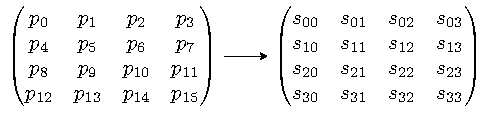
\includegraphics{../pics/aes/state.pdf}
\end{figure}    

\begin{itemize}
    \item Các phép biến đổi Add Round Key, Substitute Bytes, Shift Rows, Mix Columns được thực hiện trên ma trận $4 \times 4$ này
    \item Các phép tính số học trong AES được thực hiện trong $GF(2^8)$ với đa thức tối giản là $f(x) = x^8 + x^4 + x^3 + x + 1$
\end{itemize}

\section{Substitute Bytes}

\subsection{Substitute Bytes}

Ta sử dụng một bảng tra cứu $16 \times 16$ (S-box).

\begin{itemize}
    \item [\underline{Bước 1}] điền các số từ 0 tới 255 theo từng hàng
    \item [\underline{Bước 2}] thay thế mối byte trong bảng bằng nghịch đảo trong $GF(2^8)$. Quy ước $(00)^{-1} = 00$
    \item [\underline{Bước 3}] với mỗi byte trong bảng, ta ký hiệu 8 bit là $b_7 b_6 b_5 b_4 b_3 b_2 b_1 b_0$. Thay thế mỗi $b_i$ bằng $b_i'$ như sau
    \[ b'_i = b_i \oplus b_{(i+4) \bmod 8} \oplus b_{(i+5) \bmod 8} \oplus b_{(i+6) \bmod 8} \oplus b_{(i+7) \bmod 8} \oplus c_i \]
    với $c_i$ là bit thứ $i$ của số $0x63$.
\end{itemize}

Việc tính trên tương đương với phép nhân trên ma trận $GF(2)$ là $B' = XB + C$

\[ \begin{bmatrix}
    b'_0 \\ b'_1 \\ b'_2 \\ b'_3 \\ b'_4 \\ b'_5 \\ b'_6 \\ b'_7
\end{bmatrix} = 
\begin{bmatrix}
    1 & 0 & 0 & 0 & 1 & 1 & 1 & 1 \\
    1 & 1 & 0 & 0 & 0 & 1 & 1 & 1 \\
    1 & 1 & 1 & 0 & 0 & 0 & 1 & 1 \\
    1 & 1 & 1 & 1 & 0 & 0 & 0 & 1 \\
    1 & 1 & 1 & 1 & 1 & 0 & 0 & 0 \\
    0 & 1 & 1 & 1 & 1 & 1 & 0 & 0 \\
    0 & 0 & 1 & 1 & 1 & 1 & 1 & 0 \\
    0 & 0 & 0 & 1 & 1 & 1 & 1 & 1
\end{bmatrix} 
\begin{bmatrix}
    b_0 \\ b_1 \\ b_2 \\ b_3 \\ b_4 \\ b_5 \\ b_6 \\ b_7
\end{bmatrix} + 
\begin{bmatrix}
    1 \\ 1 \\ 0 \\ 0 \\ 0 \\ 1 \\ 1 \\ 0
\end{bmatrix}\]

Ma trận $X$ là ma trận khả nghịch, do đó phép biến đổi S-box là song ánh (one-to-one và onto mapping).

Dựa vào bảng S-box, Substitute Bytes thực hiện như sau: mỗi byte trong ma trận state $S$ dưới dạng thập lục phân là $xy$ sẽ được thay bằng giá trị ở hàng $x$ và cột $y$ của S-box.

\subsection{Inverse Sub Bytes}

Ta cần xây dựng bảng Inverse Sub Bytes (IS-box).

Việc xây dựng bảng này giống với bảng S-box ở bước 1 và 2. Tại bước 3:

\[ b_i = b'_{(i+2) \bmod 8} \oplus b'_{(i+5) \bmod 8} \oplus b'_{(i+7) \bmod 8} \oplus d_i \]
với $d_i$ là bit thứ $i$ của số $0x05$.

\subsection{Ý nghĩa của Substitute Bytes}

Bảng S-box dùng để chống lại known-plaintext và là bước duy nhất trong 4 bước không có quan hệ tuyến tính.

\section{Shift Rows}

\subsection{Shift Rows}

Trong Shift Rows, các dòng của ma trận state được biến đổi như sau:

\begin{itemize}
    \item Dòng thứ nhất giữ nguyên
    \item Dòng 2 dịch vòng trái 1 ô
    \item Dòng 3 dịch vòng trái 2 ô
    \item Dòng 4 dịch vòng trái 3 ô
\end{itemize}

\begin{figure}[ht]
    \centering
    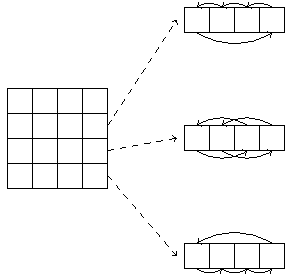
\includegraphics{../pics/aes/shiftrows.pdf}
\end{figure}

\subsection{Inverse Shift Rows}

Các dòng thứ 2, 3, 4 dịch phải tương ứng 1, 2, 3 ô.

\subsection{Ý nghĩa}

Xáo trộn các byte để tạo ra các cột cho Mix Columns.

\section{Mix Columns}

\subsection{Mix Columns}

Mix cols biến đổi từng cột của ma trận state một cách độc lập bằng phép nhân đa thức. Giả sử cột đầu tiên của ma trận state viết dưới dạng đa thức là
\[f(z) = s_{00} z^3 + s_{10} z^2 + s_{20} z + s_{30} \] với $z \in GF(2^8)$

Khi đó $f(z)$ sẽ được nhân với $a(z) = 3z^3 + z^2 + z + 2$ (tất cả hệ số, phép cộng và nhân thực hiện trên $GF(2^8)$) và sau đó modulo cho $n(z) = z^4 + 1$.

Bốn byte hệ số của kết quả sẽ thay thế cho 4 byte tương ứng trong cột. Nếu viết dưới dạng ma trận, ta có

\[ \begin{bmatrix}
    s'_{00} \\ s'_{10} \\ s'_{20} \\ s'_{30}
\end{bmatrix} = \begin{bmatrix}
    02 & 03 & 01 & 01 \\
    01 & 02 & 03 & 01 \\
    01 & 01 & 02 & 03 \\
    03 & 01 & 01 & 02
\end{bmatrix} 
\begin{bmatrix}
    s_{00} \\ s_{10} \\ s_{20} \\ s_{30}
\end{bmatrix}\]

Lưu ý rằng các số 01, 02, 03 tuy viết dưới dạng thập phân nhưng khi tính toán phải ở dạng $GF(2^8)$. Việc sử dụng 1, 2, 3 giúp tăng tốc độ tính toán vì 1 và 2 chỉ cần phép dịch bit, còn 3 là xor của 1 và 2.

\subsection{Inverse Mix Columns}

Lúc này ma trận nghịch đảo có dạng

\[\begin{bmatrix}
    \text{0E} & \text{0B} & \text{0D} & \text{09} \\
    \text{09} & \text{0E} & \text{0B} & \text{0D} \\
    \text{0D} & \text{09} & \text{0E} & \text{0B} \\
    \text{0B} & \text{0D} & \text{09} & \text{0E}
\end{bmatrix}\]

\subsection{Ý nghĩa}

Mỗi cột mới chỉ phụ thuộc cột ban đầu. Cùng với sự kết hợp Shift Rows sau 1 vài vòng biến đổi, 128 bit kết quả phụ thuộc vào tất cả 128 bit ban đầu.
Từ đó tạo ra tính khuếch tán (diffusion).

\section{Add Round Key}

\subsection{Add Round Key}

128 bit của ma trận state được XOR với 128 bit của khóa con từng vòng (4 dword 32 bit). Phép biến đổi ngược của Add Round Key là chính nó.

\subsection{Ý nghĩa}

Sự kết hợp với khóa tạo ra tính làm rối (confusion).

\section{Expand Key}

\subsection{Expand Key}

Input của thao tác Expand Key là 16 byte (4 word) của khóa, sinh ra 1 mảng 44 word (176 byte) sử dụng cho 11 vòng AES, mỗi vòng 4 word.

\begin{figure}[ht]
    \centering
    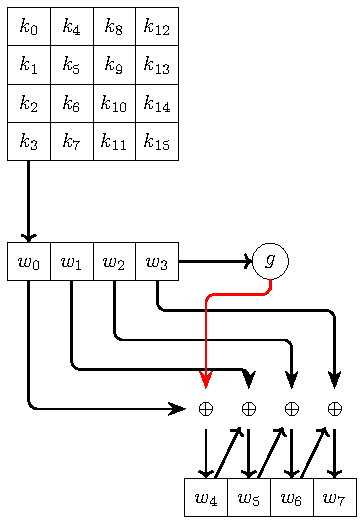
\includegraphics{../pics/aes/expandkey.pdf}
\end{figure}

Từ 4 word đầu vào $w_0 w_1 w_2 w_3$, lần lặp đầu sinh ra $w_4 w_5 w_6 w_7$, lần lặp thứ hai sinh ra $w_8 w_9 w_{10} w_{11}$, \dots

\begin{algorithmic}
    \If{$i \bmod 4 = 0$}
        \State $g \gets SubWord(RotWord(w_{i-1})) \oplus Rcon[i/4]$

        \State $w_i = w_{i-4} \oplus g$
    \Else
        \State $w_i = w_{i-4} \oplus w_{i-1}$
    \EndIf
\end{algorithmic}

Trong đó, 
\begin{itemize}
    \item $RotWord$ dịch vòng trái 1 bit, nghĩa là $b_0 b_1 b_2 \rightarrow b_1 b_2 b_0$.
    \item $SubWord$ thay mỗi byte trong word bằng bảng S-box
    \item $Rcon$ là 1 mảng hằng số gồm 10 word tương ứng với 10 vòng AES. 4 byte của một phần tử $Rcon[j]$ là $RC[j], 0, 0, 0$ với $RC[j]$ là mảng 10 byte như sau
    \begin{center}
        \begin{tabular}{|c|c|c|c|c|c|c|c|c|c|c|}
            \hline
            $j$ & 1 & 2 & 3 & 4 & 5 & 6 & 7 & 8 & 9 & 10 \\
            \hline
            $RC[j]$ & 1 & 2 & 4 & 8 & 10 & 20 & 40 & 80 & 18 & 36 \\
            \hline
        \end{tabular}
    \end{center}
    
\end{itemize}

\subsection{Ý nghĩa của Expand Key}

Dùng để chống lại known-plaintext (giống Sub Bytes dùng S-box). Đặc điểm của Expand Key gồm:

\begin{itemize}
    \item Biết một số bit của khóa hay khóa con không thể tính được các bit còn lại
    \item KHÔNG THỂ tính ngược
    \item Khuếch tán: mỗi bit của khóa chính tác động lên tất cả khóa con
\end{itemize}

\section{Kết luận}

Mã hóa AES đơn giản và có thể chạy trên các chip 8 bit.

AES cung cấp 3 biến thể cho độ dài khóa là:

\begin{itemize}
    \item 128 bit: 44 word 4 byte cho 10 vòng (11 lần ARK)
    \item 192 bit: 52 word 4 byte cho 12 vòng (13 lần ARK)
    \item 256 bit: 60 word 4 byte cho 14 vòng (15 lần ARK)
\end{itemize}